% sec_d2.tex -- d = 2 results of the finite-coupling HT note (from phi4HT2d, 2026-10-14; readability review 2026-10-15).
% Every number here has a replay row in repro_d2.tex / results_map.md (check names d2.*, i2.*).
% Needs: amsmath, booktabs, graphicx; macros \Ds, \DE, \eps, \ii, \code of the note. Inputs: tab_d2_values.tex,
% fig_d2_DeltaE.pdf (tools/make_d2_note_inputs.py, from HT/results/HT_2d/prod1/points.csv). Cites Sak:1973oqx, Behan:2017dwr, Behan:2017emf, Belavin:1984vu.
\section{Two dimensions}\label{d2:sec}

\subsection{Modes, sectors and couplings}\label{d2:modes}
In $d=2$ the exponent $s$ of the long-range interaction fixes $\Ds=(d-s)/2=1-s/2$, so $\eps=2s-2=2-4\Ds$. The
interacting window is $1<s<s_*$, that is $\frac18<\Ds<\frac12$. Its upper end is the crossover to the short-range Ising
CFT, at $s_*=2-\eta_{\rm SR}=\frac74$~\cite{Sak:1973oqx,Behan:2017dwr,Behan:2017emf}. At $s=s_*$ the fixed point is the
short-range Ising CFT decoupled from a generalized free field~\cite{Behan:2017dwr,Behan:2017emf}, so there $\DE=1$, the
dimension of the energy operator of the two-dimensional Ising model~\cite{Belavin:1984vu}. The scan covers
$\frac18\le\Ds<\frac12$.

The modes are $k=(a,b)$, $a,b\ge0$, of Eq.~\eqref{eq:weights}: the oscillator $a_{ab}$ has level $\kappa=a+b$, spin
$j=a-b$ and weight $u_{ab}^2=(\Ds)_a(\Ds)_b/(a!\,b!)$. With $f_{ab}=e^{-\ii(a-b)\vartheta}$, the two-point function of
the field~\eqref{eq:modes} is the cylinder covariance $z^{\Ds}|1-z\,e^{\ii\vartheta}|^{-2\Ds}$, with $z=e^{-\tau}$ the
radial-time variable and $\vartheta$ the angle on the circle. The oscillator $a_{00}$ is the zero mode of
Eq.~\eqref{eq:split}, and all others form the bath. A bath state with occupations $n_{ab}$ has level, particle number
and spin
\begin{equation}
 \ell=\sum_{(a,b)\neq(0,0)}(a+b)\,n_{ab},\qquad P=\sum n_{ab},\qquad J=\sum(a-b)\,n_{ab}.
\end{equation}
We keep every bath state with $\ell\le N$, with no limit on $P$ (Section~\ref{sec:split}). The scalar spectrum is
computed at $J=0$, in the sector even under the reflection $a\leftrightarrow b$. Since $\ell-J=2\sum b\,n_{ab}$ is
even, every scalar bath state has even level. The truncations at $N=2m$ and $2m+1$ therefore coincide, and we use the
even cutoffs $N=8,10,\dots,24$.

The vertices $W_j=\langle{:}\chi^j{:}\rangle$ of Eq.~\eqref{eq:Hsplit} are built exactly in the retained scalar space.
With $B=\sum_{(a,b)\neq(0,0)}u_{ab}\,a_{ab}$ the annihilation part of $\chi$ at $\vartheta=0$, and $S$ the embedding of
the scalar space,
\begin{equation}
 W_j=\sum_{i=0}^{j}\binom ji\,(B^iS)^\dagger(B^{j-i}S).
 \label{d2:eq:W}
\end{equation}
Between two scalar states the average over the circle equals the value at $\vartheta=0$, so no further projection is
needed; states of nonzero spin enter as intermediate states. Since $B$ lowers the level, $B^{j-i}S$ stays inside the
space $\ell\le N$, and the matrix elements are exact: no intermediate state is cut off.

The couplings are parametrized by $\theta=(\theta_0,\theta_1)$,
\begin{equation}
 g=\frac{192\,e^{3\theta_1}}{\Ds^2},\qquad A=\frac{4\,e^{2\theta_1}\theta_0}{\Ds},\qquad
 r=A+\frac g2-\frac{\Ds}4 ,
 \label{d2:eq:theta}
\end{equation}
with $A$ the coefficient of $q^2$ in $H_z$, Eq.~\eqref{eq:Hz}. The two tuning conditions of Eq.~\eqref{eq:tune},
$E_\sigma-E_v=\Ds$ and $E_{\phi^3}-E_v=2-\Ds$, fix $\theta$, and the prediction is $\DE=E_\varepsilon-E_v$.

\subsection{Zero-mode basis and window}\label{d2:basis}
The zero-mode basis is the density basis of Section~\ref{sec:zerobasis}, Eq.~\eqref{eq:rho}, with the training cutoff
$N_t=6$. The teacher is an energy-basis calculation at $N=6$ with 24 states per parity, taken from an auxiliary
oscillator basis of $N_{\rm osc}=192$ states. Each stored basis keeps the 20 leading eigenvectors of $\rho$ per parity,
which contain the nested bases of $n_z=12$, 16 and 20 states. Production uses $n_z=16$, and $n_z=20$ and 12 are
recomputed at every cutoff as checks. For ten values of $\Ds$ the stored bases are those of the package; for
$\Ds=0.125$, 0.135 and 0.175 new ones were trained with the same settings. No basis is transferred between values of
$\Ds$. Over all chains and cutoffs,
\begin{equation*}
 |\DE(n_z{=}20)-\DE(n_z{=}16)|\le9.4\times10^{-11},\qquad |\DE(n_z{=}12)-\DE(n_z{=}16)|\le5.2\times10^{-7},
\end{equation*}
the latter at $\Ds=0.125$, $N=22$. Three reference points at $N=14$ ($\Ds=0.126$, 0.25 and 0.4) use instead the energy
basis with 32 states per parity, recomputed at every coupling from $N_{\rm osc}=256$; they agree with $n_z=16$ to
$10^{-9}$.

The window is the consistent correction of Section~\ref{sec:window}, Eqs.~\eqref{eq:window} and~\eqref{eq:Ev}. Every
bath state of level $\ell$ is shifted by $D(\ell)=E_v(N)-E_v(N-\ell)$. The vacua $E_v(M)$, $M=0,2,\dots,N$, are computed
with their own windows, at the same couplings and in the same zero-mode basis; they are not retuned. Their fixed points
are solved as in Section~\ref{sec:window} and accepted at $10^{-11}$, and the derivatives~\eqref{eq:dEv} enter the
tuning Jacobian. The other acceptance thresholds are a tuning residual $\le1.5\times10^{-10}$, an eigenvector residual
$\le10^{-8}$ and an orthogonality defect $\le10^{-9}$. Every shipped record passes them (check \code{d2.records.gates}).

\subsection{Campaign}\label{d2:campaign}
Thirteen chains, $\Ds\in\{0.125,0.126,0.135,0.15,0.175,0.2,0.25,0.3,0.35,0.4,0.45,0.475,0.495\}$, ran from $N=8$ to 24
in steps of two on Expanse (SDSC), one chain per 64-core, 64\,GB allocation. Each cutoff was seeded by the previous one,
and the first by the package's $N=8$ reference solution or by the teacher. The 348 records (main runs, basis checks and
reference points) took $1.1\times10^4$ core-hours; a point at $N=24$ took 0.6--11\,h and up to 24\,GiB. The code is
\code{lri\_2d\_window\_hpc} at commit 889a968, and every record carries a hash of that source. The Python environment
was frozen (Python 3.11.5, NumPy 2.3.5, SciPy 1.17.0, Numba 0.65.1). The lowest value, $\Ds=0.125$, is the crossover
point $s=s_*$, where $\DE=1$.

\subsection{Finite-cutoff behaviour}\label{d2:finiteN}
Table~\ref{d2:tab:values} and Fig.~\ref{d2:fig:DE} give $\DE(N)$. All of them are values of the truncated model at that
cutoff (status: \emph{finite-$N$}). Nine cutoffs up to $N=24$ are too few, and the behaviour varies too much with $\Ds$,
for a controlled extrapolation, so we quote no continuum value in $d=2$. Steps are taken between successive cutoffs,
$\delta(N)=\DE(N)-\DE(N-2)$.
\begin{itemize}
\item $\Ds\ge0.45$: the last step $\delta(24)$ is $2.54\times10^{-6}$, $1.28\times10^{-6}$ and $1.57\times10^{-7}$ at
 0.45, 0.475 and 0.495, and the steps shrink by 18--22\% per step.
\item $0.25\le\Ds\le0.4$: $\DE$ rises monotonically, with last steps $4.30\times10^{-4}$, $3.80\times10^{-4}$,
 $2.16\times10^{-4}$ and $5.86\times10^{-5}$, which shrink by $1-(\delta(24)/\delta(16))^{1/4}=16$, 13, 11 and 8\% per
 step. If the rise continues, $\DE(24)$ bounds the limit of the truncated model from below.
\item $\Ds=0.2$: the steps change sign ($+$ up to $N=22$, $-4.2\times10^{-5}$ at $N=24$), so $\DE$ is not monotone.
\item $0.125\le\Ds\le0.175$: $\DE$ falls from $N=10$ on, and the steps grow. The last step is $-1.05\times10^{-3}$ at
 0.175 ($N=24$) and $-2.02\times10^{-2}$ at 0.125 ($N=22$), each larger than the previous one. At $\Ds=0.125$ the value
 at $N=22$, 0.9400, lies $6\%$ below the exact value 1 and moves away from it. This is the failure toward the
 short-range end discussed in Section~\ref{d2:caveats}.
\end{itemize}

\subsection{No solution at \texorpdfstring{$N=24$}{N=24} for \texorpdfstring{$\Ds=0.125$, 0.126}{small Delta sigma}: a fold}\label{d2:fold}
At $\Ds=0.125$ and 0.126 the Newton solve at $N=24$ did not converge. It was started from the $N=22$ root and from the
linear extrapolation $2\theta(22)-\theta(20)$, and repeated with a finite-difference Jacobian. Each time the residual
stalled on a floor, at $2.9\times10^{-3}$ and $2.0\times10^{-3}$. At the accepted roots of smaller $N$ the condition
number of the tuning Jacobian grows, from 84 at $N=12$ to 888 at $N=22$ ($\Ds=0.125$).

To decide whether a root exists, we scanned the valley of the residual. Write the conditions as
\begin{equation}
 f_1(\theta)=E_\sigma-E_v-\Ds,\qquad f_2(\theta)=E_{\phi^3}-E_v-(2-\Ds).
\end{equation}
At six values $\theta_0\in\{12.5,13.25,\theta_0^{\rm best},14.3,14.8,15.5\}$ around the best point of the Newton solves,
a secant iteration in $\theta_1$ solves $f_2=0$ to $|f_2|\le10^{-9}$, and we record $f_1$ there. Code, basis and solver
settings are those of production, with $n_z=16$. At $\theta_0^{\rm best}$ the first evaluation, before the secant,
reproduces the stalled residual: $\max(|f_1|,|f_2|)=2.93\times10^{-3}$ and $1.99\times10^{-3}$. A root would show as a
sign change of $f_1$ along the curve $f_2=0$. There is none: $f_1>0$ at every point (smallest value
$1.60\times10^{-3}$), with an interior minimum and a steep rise on both sides. A quartic fit in $\theta_0$ puts the
minimum at $f_1=2.686\times10^{-3}$ ($\theta_0\approx14.03$) for $\Ds=0.125$ and at $1.556\times10^{-3}$
($\theta_0\approx14.06$) for 0.126. Both are far above the effect of the zero-mode truncation ($\le5\times10^{-7}$) and
the eigensolver accuracy.

Hence, on the scanned range of $\theta_0$, the two tuning conditions have no solution at $N=24$ on the branch continued
from smaller $N$. This is a statement about the truncated model at $N=24$ and involves no extrapolation in $N$. The
minimum falls by $1.13\times10^{-3}$ per $0.001$ in $\Ds$. Near a saddle-node (fold) it is linear in the parameter,
which places the fold at
\begin{equation}
 \Ds^{\rm fold}(N=24)\approx0.1274,
\end{equation}
an estimate from two values of $\Ds$. Roots exist above it ($\Ds=0.135$ converged at $N=24$), and at $N=22$ they exist
down to 0.125. The fold has therefore moved past 0.125 between $N=22$ and 24, and the growing condition number at the
roots is its precursor. The $d=2$ data at $\Ds=0.125$ and 0.126 end at $N=22$.

\subsection{Weak coupling and the \texorpdfstring{$\epsilon$}{epsilon} expansion of the model}\label{d2:weak}
Expanded in $\eps$, the truncated model agrees with the consistent-window scheme of the perturbative calculation
(\code{HT\_Pert/}). At $\Ds=0.495$ ($\eps=0.02$) the $[4/4]$ Pad\'e approximant of that scheme's coefficients
$C_0(N),\dots,C_8(N)$ reproduces $\DE(N)$ to $9.4\times10^{-12}$ at every $N=8,\dots,24$, and at $\Ds=0.475$
($\eps=0.1$) to $7.6\times10^{-8}$ (check \code{d2.pert\_consistent}). A difference $\delta C_4$ in the fourth-order
coefficient would show as $\delta C_4\,\eps^4$, so $|\delta C_4|\lesssim6\times10^{-5}$ at every $N\le24$. In that
scheme the fourth-order coefficient grows with the cutoff, $C_4(N)\simeq5.003-\frac{365}{4374\pi}\ln N$, that is like
$-0.027\ln N$ (exact sums to $N=2000$ in \code{HT\_Pert/}), while the continuum value $C_4(2)$ is finite. The $d=2$
window model is thus known to be correct only through third order in $\eps$. In the perturbative calculation a larger
correction, the complete window of \code{HT\_Pert/}, removes this logarithm; it has no finite-coupling counterpart here.

\begin{table}[t]
\centering\small\setlength{\tabcolsep}{4.5pt}
\begin{tabular}{@{}l l l l l l l l@{}}
\toprule
$\Delta_\sigma$ & $s$ & $N=16$ & $N=20$ & $N=22$ & $N=24$ & last step & behaviour\\
\midrule
0.125 & 1.75 & 0.98916082 & 0.96025057 & 0.94002832 & n.s. & $-2.02\times10^{-2}$ & falls; steps grow\\
0.126 & 1.748 & 0.99053540 & 0.96363343 & 0.94568294 & n.s. & $-1.80\times10^{-2}$ & falls; steps grow\\
0.135 & 1.73 & 0.99948557 & 0.98399079 & 0.97537120 & 0.96202900 & $-1.33\times10^{-2}$ & falls; steps grow\\
0.15 & 1.7 & 1.00548133 & 0.99836315 & 0.99471461 & 0.99022622 & $-4.49\times10^{-3}$ & falls; steps grow\\
0.175 & 1.65 & 1.00330217 & 1.00162583 & 1.00076308 & 0.99971675 & $-1.05\times10^{-3}$ & falls; steps grow\\
0.2 & 1.6 & 0.99490861 & 0.99526003 & 0.99534664 & 0.99530455 & $-4.21\times10^{-5}$ & not monotone\\
0.25 & 1.5 & 0.97541470 & 0.97674862 & 0.97727730 & 0.97770747 & $+4.30\times10^{-4}$ & rises; shrink 16\%/step\\
0.3 & 1.4 & 0.96158682 & 0.96267180 & 0.96311194 & 0.96349241 & $+3.80\times10^{-4}$ & rises; shrink 13\%/step\\
0.35 & 1.3 & 0.95679429 & 0.95736832 & 0.95760910 & 0.95782471 & $+2.16\times10^{-4}$ & rises; shrink 11\%/step\\
0.4 & 1.2 & 0.96152920 & 0.96167002 & 0.96173269 & 0.96179129 & $+5.86\times10^{-5}$ & rises; shrink 8\%/step\\
0.45 & 1.1 & 0.97526784 & 0.97527566 & 0.97527858 & 0.97528111 & $+2.54\times10^{-6}$ & small steps\\
0.475 & 1.05 & 0.98580651 & 0.98581110 & 0.98581268 & 0.98581396 & $+1.28\times10^{-6}$ & small steps\\
0.495 & 1.01 & 0.99678104 & 0.99678155 & 0.99678174 & 0.99678190 & $+1.57\times10^{-7}$ & small steps\\
\bottomrule
\end{tabular}

\caption{$\DE(N)$ in $d=2$ at finite coupling ($n_z=16$, consistent window): finite-$N$ values of the truncated model,
not continuum values. n.s.: no solution at $N=24$ (Section~\ref{d2:fold}). Last step: between the two largest cutoffs.
Shrink: $1-(\delta(24)/\delta(16))^{1/4}$.}
\label{d2:tab:values}
\end{table}

\begin{figure}[t]
\centering
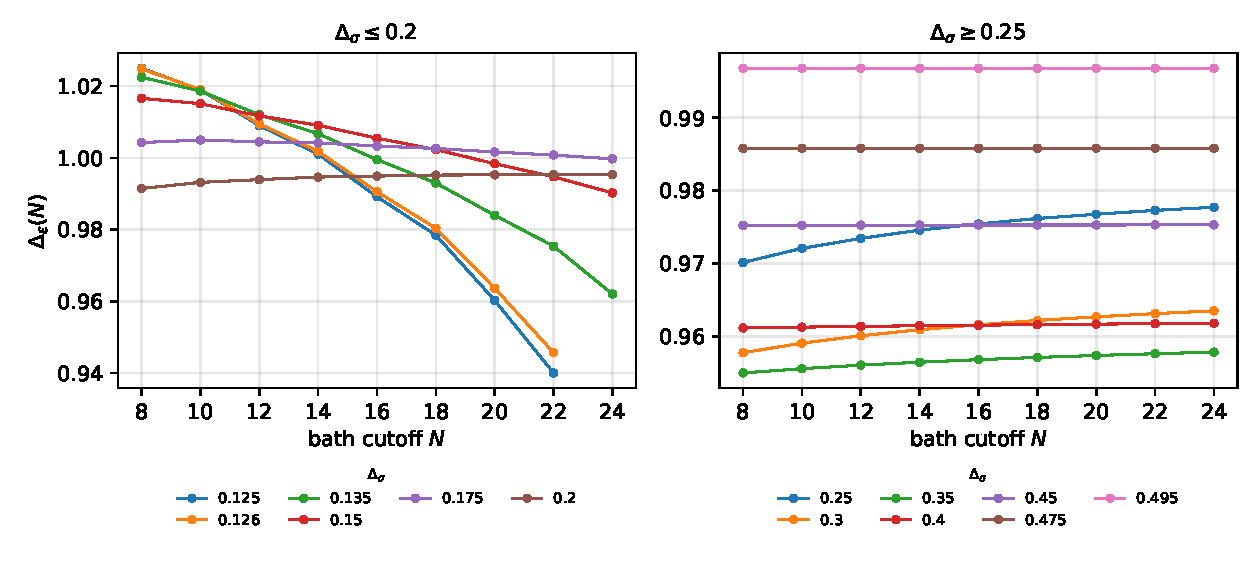
\includegraphics[width=\textwidth]{fig_d2_DeltaE.pdf}
\caption{$\DE(N)$ in $d=2$ against the bath cutoff $N$, for the 13 values of $\Ds$ (made by
\code{tools/make\_d2\_note\_inputs.py} from \code{HT/results/HT\_2d/prod1/points.csv}).}
\label{d2:fig:DE}
\end{figure}
